\documentclass[notes=show]{beamer}
\usepackage{amsmath,amsfonts}
\usetheme{Madrid}
\usecolortheme{seagull}
\setbeamertemplate{navigation symbols}{}
\begin{document}
\title{GMM, Indirect Inference and Bootstrap}
\subtitle{Instrumental variables}
\author[Willi Mutschler]{Willi Mutschler}
\date{Winter 2015/2016}
\institute{TU Dortmund}
\maketitle

\section{Instrumental variables}
\begin{frame}\frametitle{TO IMPROVE}
  \begin{itemize}
    \item Slide with inconsistency and forecastablity? Do you really need it?
    \item Make the structure and dimensions of $W$, $W'u$, $W_t$, $W_t'u_t$ more clear
    \item Interpretations and structures of $M_X$, $P_W$
  \end{itemize}
\end{frame}


\begin{frame}\frametitle{Instrumental variables}\framesubtitle{Preliminaries}
\begin{itemize}
    \item OLS is not consistent and biased if $E\left( u_{t}|X_{t}\right) \neq 0$
    \item Define an information set $\Omega _{t}$ (a $\sigma $-algebra), such that
    \begin{equation*}
    E\left( u_{t}|\Omega _{t}\right) =0
    \end{equation*}
    \item This rationality conditions or moment conditions can be used for estimation
    \item Variables in $\Omega _{t}$ are called \textbf{instrumental variables}
    \newline
    (or instruments)
    \item We denote the instrument vector by $W_{t}$
\end{itemize}
\end{frame}


\begin{frame}\frametitle{Instrumental variables}\framesubtitle{Correlation between errors and disturbances (I)}
Errors in variables (e.g. in questionnaires)
\begin{itemize}
    \item Consider the model
    \begin{equation*}
        y_{t}=\alpha +\beta x_{t}^{\ast }+\varepsilon _{t},\quad \varepsilon_{t}\sim iid(0,\sigma _{\varepsilon }^{2})
    \end{equation*}
    \item The exogenous variable $x_{t}^{\ast }$ is unobservable
    \item We can only observe
    \begin{equation*}
        x_{t}=x_{t}^{\ast }+v_{t}
    \end{equation*}%
    where $v_{t}\sim iid(0,\sigma _{v}^{2})$ are independent of everything else
    \item Estimators of $y_{t}=\alpha +\beta x_{t}+u_{t}$ are inconsistent\hfill\lbrack P]
\end{itemize}
\end{frame}


\begin{frame}\frametitle{Instrumental variables}\framesubtitle{Correlation between errors and disturbances (II)}
Omitted variables bias
\begin{itemize}
    \item Let
    \begin{equation*}
        y_{t}=\alpha +\beta _{1}x_{1t}+\beta _{2}x_{2t}+\varepsilon _{t}
    \end{equation*}
    \item If $x_{2}$ is unobservable, one estimates
    \begin{equation*}
        y_{t}=\alpha +\beta _{1}x_{1t}+u_{t}
    \end{equation*}
    where $u_{t}=\beta _{2}x_{2t}+\varepsilon _{t}$
    \item If $x_{2t}$ and $x_{1t}$ are correlated then so are $u_{t}$ and $x_{1t} $
\end{itemize}
\end{frame}


\begin{frame}\frametitle{Instrumental variables}\framesubtitle{Correlation between errors and disturbances (III)}
Endogeneity
\begin{itemize}
    \item Standard example: supply and demand curves determine both price and quantity
    \begin{eqnarray*}
        q_{t} &=&\gamma _{d}p_{t}+X_{t}^{d}\beta _{d}+u_{t}^{d} \\
        q_{t} &=&\gamma _{s}p_{t}+X_{t}^{s}\beta _{s}+u_{t}^{s}
    \end{eqnarray*}
    \item Solve for $q_{t}$ and $p_{t}$
    \begin{equation*}
        \left[
        \begin{array}{c}
        q_{t} \\
        p_{t}
        \end{array}
        \right] =\left[
        \begin{array}{ll}
        1 & -\gamma _{d} \\
        1 & -\gamma _{s}
        \end{array}
        \right] ^{-1}\left( \left[
        \begin{array}{c}
        X_{t}^{d}\beta _{d} \\
        X_{t}^{s}\beta _{s}
        \end{array}
        \right] +\left(
        \begin{array}{c}
        u_{t}^{d} \\
        u_{t}^{s}
        \end{array}
        \right) \right)
    \end{equation*}
\end{itemize}
\end{frame}


\begin{frame}\frametitle{Instrumental variables}\framesubtitle{Correlation between errors and disturbances (III)}
\begin{itemize}
    \item Since $q_{t}$ and $p_{t}$ depend on both $u_{t}^{d}$ and $u_{t}^{s}$single equation OLS estimation of
    \begin{eqnarray*}
        q_{t} &=&\gamma _{d}p_{t}+X_{t}^{d}\beta _{d}+u_{t}^{d} \\
        q_{t} &=&\gamma _{s}p_{t}+X_{t}^{s}\beta _{s}+u_{t}^{s}
    \end{eqnarray*}
    is inconsistent
    \item The right hand side variable $p_{t}$ is correlated with the error term
    \item The condition $E\left( u_{t}|\Omega _{t}\right) =0$ is violated if $p_{t}$ is in $\Omega _{t}$
\end{itemize}
\end{frame}


\begin{frame}\frametitle{Instrumental variables}\framesubtitle{Correlation between errors and disturbances}
\begin{itemize}
    \item \textbf{Warning! }Inconsistency is not always a problem
    \item If we simply want to forecast, we can use inconsistent estimators
    \item Trivial example:\vspace*{-0.3cm}
\end{itemize}
\begin{center}
    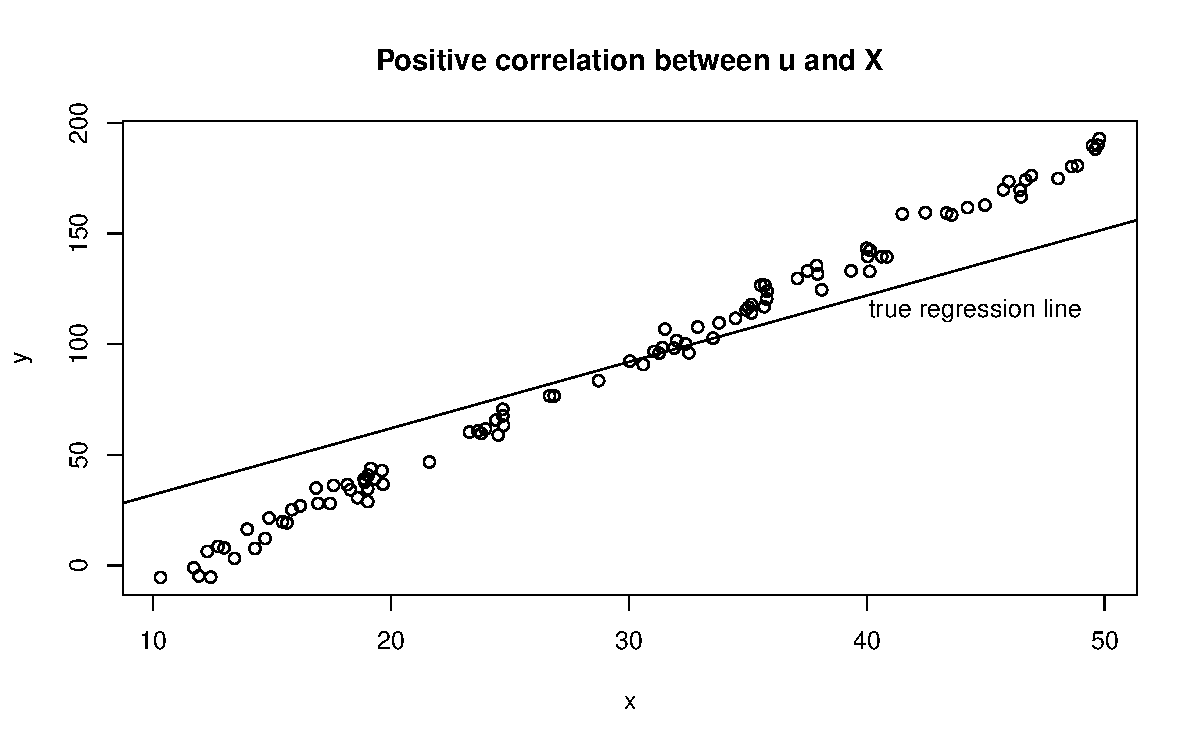
\includegraphics[width=7cm]{plots/forecasting.pdf}
\end{center}
\end{frame}


\begin{frame}\frametitle{Instrumental variables}\framesubtitle{The simple IV estimator}
\begin{itemize}
    \item Let $W$ denote the $T\times K$ matrix of instruments
    \item All columns of $X$ with $X_{t}\in \Omega _{t}$ should be included in $ W $
    \item Then $E\left( u_{t}|W_{t}\right) =0$ implies the moment condition
    \begin{equation*}
        E\left( W^{\prime }u\right) =E\left( W^{\prime }\left( y-X\beta \right)\right) =0
    \end{equation*}
    \item The IV estimator is a method of moment estimator
    \item The solution is
    \begin{equation*}
        \hat{\beta}_{IV}=\left( W^{\prime }X\right) ^{-1}W^{\prime }y
    \end{equation*}
\end{itemize}
\end{frame}


\begin{frame}\frametitle{Instrumental variables}\framesubtitle{Properties}
\begin{itemize}
    \item The simple IV estimator is consistent if
    \begin{equation*}
        \textsl{plim}\frac{1}{n}W^{\prime }X=S_{WX}
    \end{equation*}
    is deterministic and nonsingular\hfill \lbrack P]
    \item The simple IV estimator is asymptotically normal,
    \begin{equation*}
        \sqrt{n}\left( \hat{\beta}_{IV}-\beta \right) \rightarrow U\sim N\left(0,\sigma ^{2}\left( S_{WX}\right) ^{-1}S_{WW}\left( S_{WX}^{\prime }\right)^{-1}\right)
    \end{equation*}
    where $S_{WW}=\textsl{plim}\frac{1}{n}W^{\prime }W$\hfill \lbrack P]
\end{itemize}
\end{frame}


\begin{frame}\frametitle{Instrumental variables}\framesubtitle{How to find instruments}
\begin{itemize}
    \item Instruments must be
    \begin{enumerate}
        \item exogenous, i.e. $\textsl{plim}\frac{1}{n}W^{\prime }u=0$
        \item valid, i.e. $\textsl{plim}\frac{1}{n}W^{\prime }X=S_{WX}$ non-singular
    \end{enumerate}
    \item Natural experiments (weather, earthquakes, \ldots )
    \item Angrist and Pischke (2009):
\end{itemize}
\begin{quotation}
    Good instruments come from a combination of institutional knowledge and ideas about the processes determining the variable of interest.
\end{quotation}
\end{frame}


\begin{frame}\frametitle{Instrumental variables}\framesubtitle{How to find instruments}
\begin{examples}
    Natural experiments
    \begin{enumerate}
        \item Br\"{u}ckner and Ciccone: Rain and the demographic window of opportunity, Econometrica 79 (2011) 923-947
        \item Angrist and Evans: Children and their parents' labor supply: Evidence from exogenous variation in family size, American Economic Review 88 (1998) 450-77.
    \end{enumerate}
\end{examples}
\end{frame}
\note{\begin{itemize}
  \item Negative ökonomische EK-Schocks können für demokratische Verbesserung Instrumente liefern (ökonomische Rezessionen), Sub-Sahara Afrikanische Länder, INstrument: Negative Regenschocks
  \item Endogenität von Fertilität, Arbeitsentscheidung nach Geburt. Effekt von Kindergeburt auf Arbeitsangebot. Instrument: Präferenz für mixed Kinder-Komposition, Eltern mit 2 Mädels probieren noch mal für Jungen.
\end{itemize}}

\begin{frame}\frametitle{Instrumental variables}\framesubtitle{How to find instruments}
\begin{examples}
    Institutional arrangements
    \begin{enumerate}
        \item Angrist and Krueger: Does Compulsory School Attendance Affect Schooling and Earnings?, Quarterly Journal of Economics 106 (1991) 979-1014.
        \item Levitt: The Effect of Prison Population Size on Crime Rates: Evidence from Prison Overcrowding Litigation, Quarterly Journal of Economics 111 (1996) 319-351.
    \end{enumerate}
\end{examples}
\end{frame}
\note{\begin{itemize}
  \item Welcher Monat man geboren ist: Keine Korrelation mit Fähigkeit und Earnings, keine determinante von Fähigkeiten, aber korreliert mit years of schooling. Männer die gezwungen werden zur Schule zu gehen, verdienen meht
  \item Gerichtsverfahren. Simultanität/Endogenität zwischen Gefängnisbevölkerung und Verbrechensraten. Ideee: Gefängnisbevölkerung steigt impliziert sinkende Verbrechensrate. Messfehler. IV: Korreliert mit Verändung Gef.Bevölkerung aber sonst unrelated to crime rates, state prison overcroding litigation.
\end{itemize}}

\begin{frame}\frametitle{Instrumental variables}\framesubtitle{How to find instruments}
\begin{itemize}
    \item In a time series context, one can sometimes use lagged endogenous regressors as instrumental variables
    \item Example:
    \begin{equation*}
        y_{t}=\alpha +\beta x_{t}+u_{t}
    \end{equation*}%
    with $E(u_{t}|x_{t})\neq 0$
    \item If $Cov\left( x_{t},x_{t-1}\right) \neq 0$ but $Cov\left(u_{t},x_{t-1}\right) =0$,\newline
    then $x_{t-1}$ can be used as instrumental variable
    \item Attention: $Cov\left( u_{t},x_{t-1}\right) =0$ is not always obvious
\end{itemize}
\end{frame}


\begin{frame}\frametitle{Instrumental variables}\framesubtitle{How to find instruments}
\begin{example}[Measurement error in time series]
    Consider the model
    \begin{eqnarray*}
        y_{t} &=&\alpha +\beta x_{t}^{\ast }+u_{t} \\
        x_{t}^{\ast } &=&\rho x_{t-1}^{\ast }+\varepsilon _{t} \\
        x_{t} &=&x_{t}^{\ast }+v_{t}.
    \end{eqnarray*}
    Then $x_{t-1}$ is a valid instrument for a regression of $y_{t}$ on $x_{t}$,\newline
    and $\alpha $ and $\beta $ will be estimated consistently.
\end{example}
\hfill [\texttt{IVLags.R}]
\end{frame}


\begin{frame}\frametitle{Instrumental variables}\framesubtitle{How to find instruments}
\begin{example}[Omitted variable bias in time series]
    Consider the model
    \begin{eqnarray*}
        y_{t} &=&\alpha +\beta _{1}x_{1t}+\beta _{2}x_{t2}+u_{t} \\
        x_{1t} &=&\rho _{11}x_{1,t-1}+\rho _{12}x_{2,t-1}+\varepsilon _{1t} \\
        x_{2t} &=&\rho _{21}x_{1,t-1}+\rho _{22}x_{2,t-1}+\varepsilon _{2t}
    \end{eqnarray*}%
    Then $x_{1,t-1}$ is \textbf{not} a valid instrument for a regression of $y_{t}$ on $x_{1t}$, and $\alpha $ and $\beta _{1}$ will \textbf{not} be estimated consistently.
\end{example}
\hfill [\texttt{IVLags.R}]
\end{frame}


\begin{frame}\frametitle{Instrumental variables}\framesubtitle{How to find instruments}
\begin{example}[Endogeneity in time series]
    Consider the model
    \begin{eqnarray*}
        y_{t} &=&\alpha +\beta _{1}x_{t}+\beta _{2}y_{t-1}+u_{t} \\
        x_{t} &=&\gamma +\delta _{1}y_{t}+\delta _{2}x_{t-1}+v_{t}
    \end{eqnarray*}%
    Then $x_{1,t-1}$ is a valid instrument for a regression of $y_{t}$ on $x_{t}$ and $y_{t-1}$, and $\alpha ,\beta _{1}$ and $\beta _{2}$ will be estimated consistently.
\end{example}
\hfill [\texttt{IVLags.R}]
\end{frame}


\begin{frame}\frametitle{Instrumental variables}\framesubtitle{Generalized IV estimation}
\begin{itemize}
    \item If the number of instruments $L$ is larger than the number of parameters $K$, the model is \textbf{overidentified}
    \item Right-multiply the $T\times L$ matrix $W$ by an $L\times K$ matrix $J$ to obtain an $T\times K$ instrument matrix $WJ$
    \item Linear combinations of the instruments in $W$
    \item One can show that the asymptotically optimal matrix is $J=\left(W^{\prime }W\right) ^{-1}W^{\prime }X$, see Davidson and MacKinnon.
\end{itemize}
\end{frame}


\begin{frame}\frametitle{Instrumental variables}\framesubtitle{Generalized IV estimation}
\begin{itemize}
    \item The generalized IV estimator is%
    \begin{eqnarray*}
        \hat{\beta}_{GIV} &=&\left( \left( WJ\right) ^{\prime }X\right) ^{-1}\left(WJ\right) ^{\prime }y \\
        &=&\left( X^{\prime }W\left( W^{\prime }W\right) ^{-1}W^{\prime }X\right)^{-1}X^{\prime }W\left( W^{\prime }W\right) ^{-1}W^{\prime }y \\
        &=&\left( X^{\prime }P_{W}X\right) ^{-1}X^{\prime }P_{W}y
    \end{eqnarray*}
    with $P_{W}=W\left( W^{\prime }W\right) ^{-1}W^{\prime }$
    \item Consistency and asymptotic normality still hold
\end{itemize}
\end{frame}


\begin{frame}\frametitle{Instrumental variables}\framesubtitle{Generalized IV estimation}
\begin{itemize}
    \item The two-stage-least-squares (2SLS) interpretation
    \item The matrix $J$ is similar to $\hat{\beta}$ in the standard OLS model,
    \begin{equation*}
        J=\left( W^{\prime }W\right) ^{-1}W^{\prime }X
    \end{equation*}
    \item Hence, $WJ$ is similar to $X\hat{\beta}$
    \item The optimal instruments are obtained if we regress the \newline
    endogenous regressors on the instruments (1st stage), and \newline
    then use the fitted values as regressors (2nd stage)
\end{itemize}
\end{frame}


\begin{frame}\frametitle{Instrumental variables}\framesubtitle{Finite sample properties}
\begin{itemize}
    \item The finite sample properties of IV estimators are complex
    \item In the overidentified case, the first $L-K$ moments exist,\newline
    but higher moments do not
    \item If the expectation exists, IV estimators are in general biased
    \item The simple IV estimator has \textbf{very} heavy tails,\newline
    even the first moment does not exist!
    \item The estimator can be extremely far off the true value
\end{itemize}
\hfill [\texttt{ivfinite.R}]

\end{frame}


\begin{frame}\frametitle{Instrumental variables}\framesubtitle{Hypothesis testing}
\begin{itemize}
    \item Exact hypothesis tests are usually not feasible
    \item Asymptotic tests are based on the asymptotic normality
    \item An estimator of the covariance matrix of $\hat{\beta}_{IV}$ is
    \begin{equation*}
        \widehat{Cov}\left( \hat{\beta}_{IV}\right) =\hat{\sigma}^{2}\left(X^{\prime }P_{W}X\right) ^{-1}
    \end{equation*}
    with
    \begin{eqnarray*}
        P_{W} &=&W\left( W^{\prime }W\right) ^{-1}W^{\prime } \\
        \hat{\sigma}^{2} &=&\frac{1}{n}\left( y-X\hat{\beta}_{IV}\right) ^{\prime}\left( y-X\hat{\beta}_{IV}\right)
    \end{eqnarray*}
\end{itemize}
\end{frame}


\begin{frame}\frametitle{Instrumental variables}\framesubtitle{Hypothesis testing}
\begin{itemize}
    \item Asymptotic $t$-test
    \begin{eqnarray*}
        H_{0} &:&\beta _{i}=\beta _{i0} \\
        H_{1} &:&\beta _{i}\neq \beta _{i0}
    \end{eqnarray*}
    \item Under the null hypothesis, the test statistic
    \begin{equation*}
        t=\frac{\hat{\beta}_{i}-\beta _{i0}}{\sqrt{\widehat{Var}\left( \hat{\beta}_{i}\right) }}
    \end{equation*}
    is asymptotically $N(0,1)$
\end{itemize}
\end{frame}


\begin{frame}\frametitle{Instrumental variables}\framesubtitle{Hypothesis testing}
\begin{itemize}
    \item Asymptotic Wald test (similiar to an $F$-test)
    \begin{equation*}
        H_{0}:\beta _{2}=\beta _{20},\quad H_{1}:\beta _{2}\neq \beta _{20}
    \end{equation*}
    where $\beta _{2}$ is a length $L$ subvector of $\beta $
    \item Under the null hypothesis, the test statistic
    \begin{equation*}
    W=\left( \hat{\beta}_{2}-\beta _{20}\right) ^{\prime }\left[ \widehat{Cov} \left( \hat{\beta}_{2}\right) \right] ^{-1}\left( \hat{\beta}_{2}-\beta_{20}\right)
    \end{equation*}
    is asymptotically $\chi ^{2}$ with $L$ degrees of freedom
\end{itemize}
\end{frame}


\begin{frame}\frametitle{Instrumental variables}\framesubtitle{Hypothesis testing}
\begin{itemize}
    \item Testing overidentifying restrictions
    \item The identifying restrictions are
    \begin{eqnarray*}
        E(u_{t}|W_{t}) &=&0 \\
        \text{or\quad }E\left( W^{\prime }u\right) &=&0
    \end{eqnarray*}
    \item If the model is just identified the validity of the restriction cannot be tested
    \item If the model is overidentified, one can test if the overidentifying restrictions hold, i.e. if the instruments are valid and exogenous
\end{itemize}
\end{frame}


\begin{frame}\frametitle{Instrumental variables}\framesubtitle{Hypothesis testing}
\begin{itemize}
    \item Basic test idea: Check if the IV residuals can be explained \newline
    by the full set of instruments
    \item Compute the IV residuals $\hat{u}$
    \item Regress the residuals on all instruments $W$
    \item Under the null hypothesis, the test statistic
    \begin{equation*}
        nR^{2}\sim \chi _{m}^{2}
    \end{equation*}
    where $m$ is the degree of overidentification
\end{itemize}
\end{frame}


\begin{frame}\frametitle{Instrumental variables}\framesubtitle{Hypothesis testing}
Davidson and MacKinnon (2004, p. 338):
\begin{quotation}
    Even if we do not know quite how to interpret a significant value of the overidentification test statistic, it is always a good idea to compute it. If it is significantly larger than it should be by chance under the null hypothesis, one should be extremely cautious in interpreting the estimates, because it is quite likely either that the model is specified incorrectly or that some of the instruments are invalid.
\end{quotation}
\end{frame}


\begin{frame}\frametitle{Instrumental variables}\framesubtitle{Hypothesis testing}
\begin{itemize}
    \item Durbin-Wu-Hausman test
    \begin{eqnarray*}
        H_{0} &:&E\left( X^{\prime }u\right) =0 \\
        H_{1} &:&E\left( W^{\prime }u\right) =0
    \end{eqnarray*}
    \item Test if IV estimation is really necessary or if OLS would do
    \item Under $H_{0}$, OLS is consistent and efficient, but IV is just consistent
    \item Under $H_{1}$, OLS is inconsistent, but IV is still consistent
    \item Basic test idea: Compare $\hat{\beta}_{OLS}$ and $\hat{\beta}_{IV}$. If they are \newline
    `too different', reject $H_{0}$
\end{itemize}
\end{frame}


\begin{frame}\frametitle{Instrumental variables}\framesubtitle{Hypothesis testing}
\begin{itemize}
    \item The difference between the estimators is
    \begin{eqnarray*}
        &&\hat{\beta}_{IV}-\hat{\beta}_{OLS} \\
        &=&\left( X^{\prime }P_{W}X\right) ^{-1}X^{\prime}P_{W}y-\left( X^{\prime}X\right) ^{-1}X^{\prime }y \\
        &=&\left( X^{\prime }P_{W}X\right) ^{-1}\left( X^{\prime}P_{W}y-\left(X^{\prime }P_{W}X\right) \left( X^{\prime }X\right) ^{-1}X^{\prime }y\right)\\
        &=&\left( X^{\prime }P_{W}X\right) ^{-1}\left( X^{\prime}P_{W}\left(I-X\left( X^{\prime }X\right) ^{-1}X^{\prime }\right) y\right)  \\
        &=&\left( X^{\prime }P_{W}X\right) ^{-1}\left( X^{\prime}P_{W}M_{X}\,y\right)
    \end{eqnarray*}
\end{itemize}
\end{frame}


\begin{frame}\frametitle{Instrumental variables}\framesubtitle{Hypothesis testing}
\begin{itemize}
    \item We need to test if $X^{\prime }P_{W}M_{X}\,y$ is significantly different from 0
    \item This term is identically equal to zero for all variables in $X$ that are instruments (i.e. that are also in $W$)
    \item Denote by $\tilde{X}$ all possibly endogenous regressors
    \item To test if $\tilde{X}^{\prime }P_{W}M_{X}\,y$ is significantly different from zero, perform a Wald test of $\delta =0$ in the regression
    \begin{equation*}
        y=X\beta +P_{W}\tilde{X}\delta +u
    \end{equation*}
\end{itemize}
\end{frame}

\end{document} 